\subsection{Modelo numérico do sistema de suspensão ativa}
Com base nas matrizes A e B do sistema linearizado obtidas em \ref{ed:linsys:ax} e \ref{ed:linsys:BuBw} e nos parâmetros na tabela \ref{tb:parametros} do Apêndice, obtemos os seguintes valores numéricos do sistema LTI que será utilizado no benchmark deste trabalho, considerou-se que o sistema é um LPV com incerteza paramétrica $\delta$ na massa do veiculo, podendo variar em $\pm 100 kg$ ao redor do valor nominal do modelo de dependendo do carregamento do veiculo:
%\ms, \mus, \bls, \bnls, \bys, \kls, \knls, \kt

\begin{equation}\label{ed:linsys:ALPV}
    \begin{split}
        \mathbf{A} =
        \begin{bmatrix}
            0 & 1 & 0 & 0 & \\            
            -\frac{\kls}{\ms+\delta}&-\frac{\bls}{\ms+\delta}&\frac{\kls}{\ms+\delta}&\frac{\bls}{\ms+\delta} &\\ \  
            0 & 0 & 0 & 1 & \\
            \frac{\kls}{\mus}&\frac{\bls}{\mus}&-\frac{(6925.1077\cdot10^{3})}{\mus}&-\frac{\bls}{\mus} &\\
        \end{bmatrix}
    \end{split}
\end{equation}

\begin{equation}\label{ed:linsys:BLPV}
    \begin{split}
        \mathbf{B_u} = 
        \begin{bmatrix}
            0 & \\            
            -\frac{1}{\ms+\delta}&\\ \\  
            0 & \\
            \frac{1}{\mus}&\\
        \end{bmatrix};
    \end{split}
    \begin{split}
        \mathbf{B_w} = 
        \begin{bmatrix}
            0 & \\            
            0 &\\ \\  
            0 & \\
            \frac{\kt}{\mus}& \\
        \end{bmatrix}
    \end{split}
\end{equation}

Para a matriz $\mathbf{C}$ consideraremos ser possível a leitura de todos os estados do sistema, e para as matrizes $D_u$ e $D_w$, consideramos que não há termo de transmissão direta das entradas, como exibido a seguir:

\begin{equation} \label{eq:matriz_c}
    \begin{split}
        \mathbf{C}=
    \end{split}
    \begin{bmatrix}
        1&0&0&0&\\
        0&1&0&0&\\
        0&0&1&0&\\
        0&0&0&1&\\
    \end{bmatrix};\ \
    \begin{split}
        \mathbf{D_u} = 0
    \end{split};\ \
    \begin{split}
        \mathbf{D_w} = 0
    \end{split};\ \ 
\end{equation}

\subsection{Especificação da região de \( \mathcal{D}\)-estabilidade desejada}
Deseja-se um valor de Máximo overshoot percentual de $M_O \leq 10$ \% e Tempo de acomodação para a faixa de tolerância de 2 \% $T_S \leq 0.5$ s. 
Dada a equação para o cálculo da taxa de amortecimento para um valor de máximo overshoot dado, obtém-se o seguinte valor objetivo para $\xi$:

\begin{equation*}
    \xi=-\frac{ln\left(0.1\right)}{\sqrt{\pi^2+ln^2(0.1)}}=0.5912
\end{equation*}

Dada a equação para o cálculo da $\omega_n$ objetivo para um tempo de assentamento dado, obtém-se o seguinte valor objetivo para $\omega_n$:

\begin{equation*}
    \omega_n=-\frac{ln\left( 0.02*\sqrt{1-0.5912} \right)}{0.5*0.5912}=13.5328
\end{equation*}

Para $\xi=0.5912$ e $\omega_n=13.5328$ os parâmetros $\sigma_p$ e $\theta$ são obtidos como se segue

\begin{equation}\label{ed:dstab:params}
    \begin{split}
       \sigma_p=-\omega_n=-13.5328\ \ rad\cdot s^{-1}\\
       \beta_p=-20\cdot\omega_n=-270.6566\ \ rad\cdot s^{-1}\\
       \theta=\pi-\cos{(\xi)}^{-1}=0.9383\ \ rad\\    
    \end{split}
\end{equation}

Apenas para limitar a região de \( \mathcal{D}\)-estabilidade desejada, tomaremos o limite a esquerda como sendo $20\cdot\sigma_p$. A região de \( \mathcal{D}\)-estabilidade definida para acomodação do sistema é exibida na figura \eqref{eq:dsta:regiaodef} a seguir:

\FloatBarrier
\begin{figure}[htbp] 
  \begin{centering}
    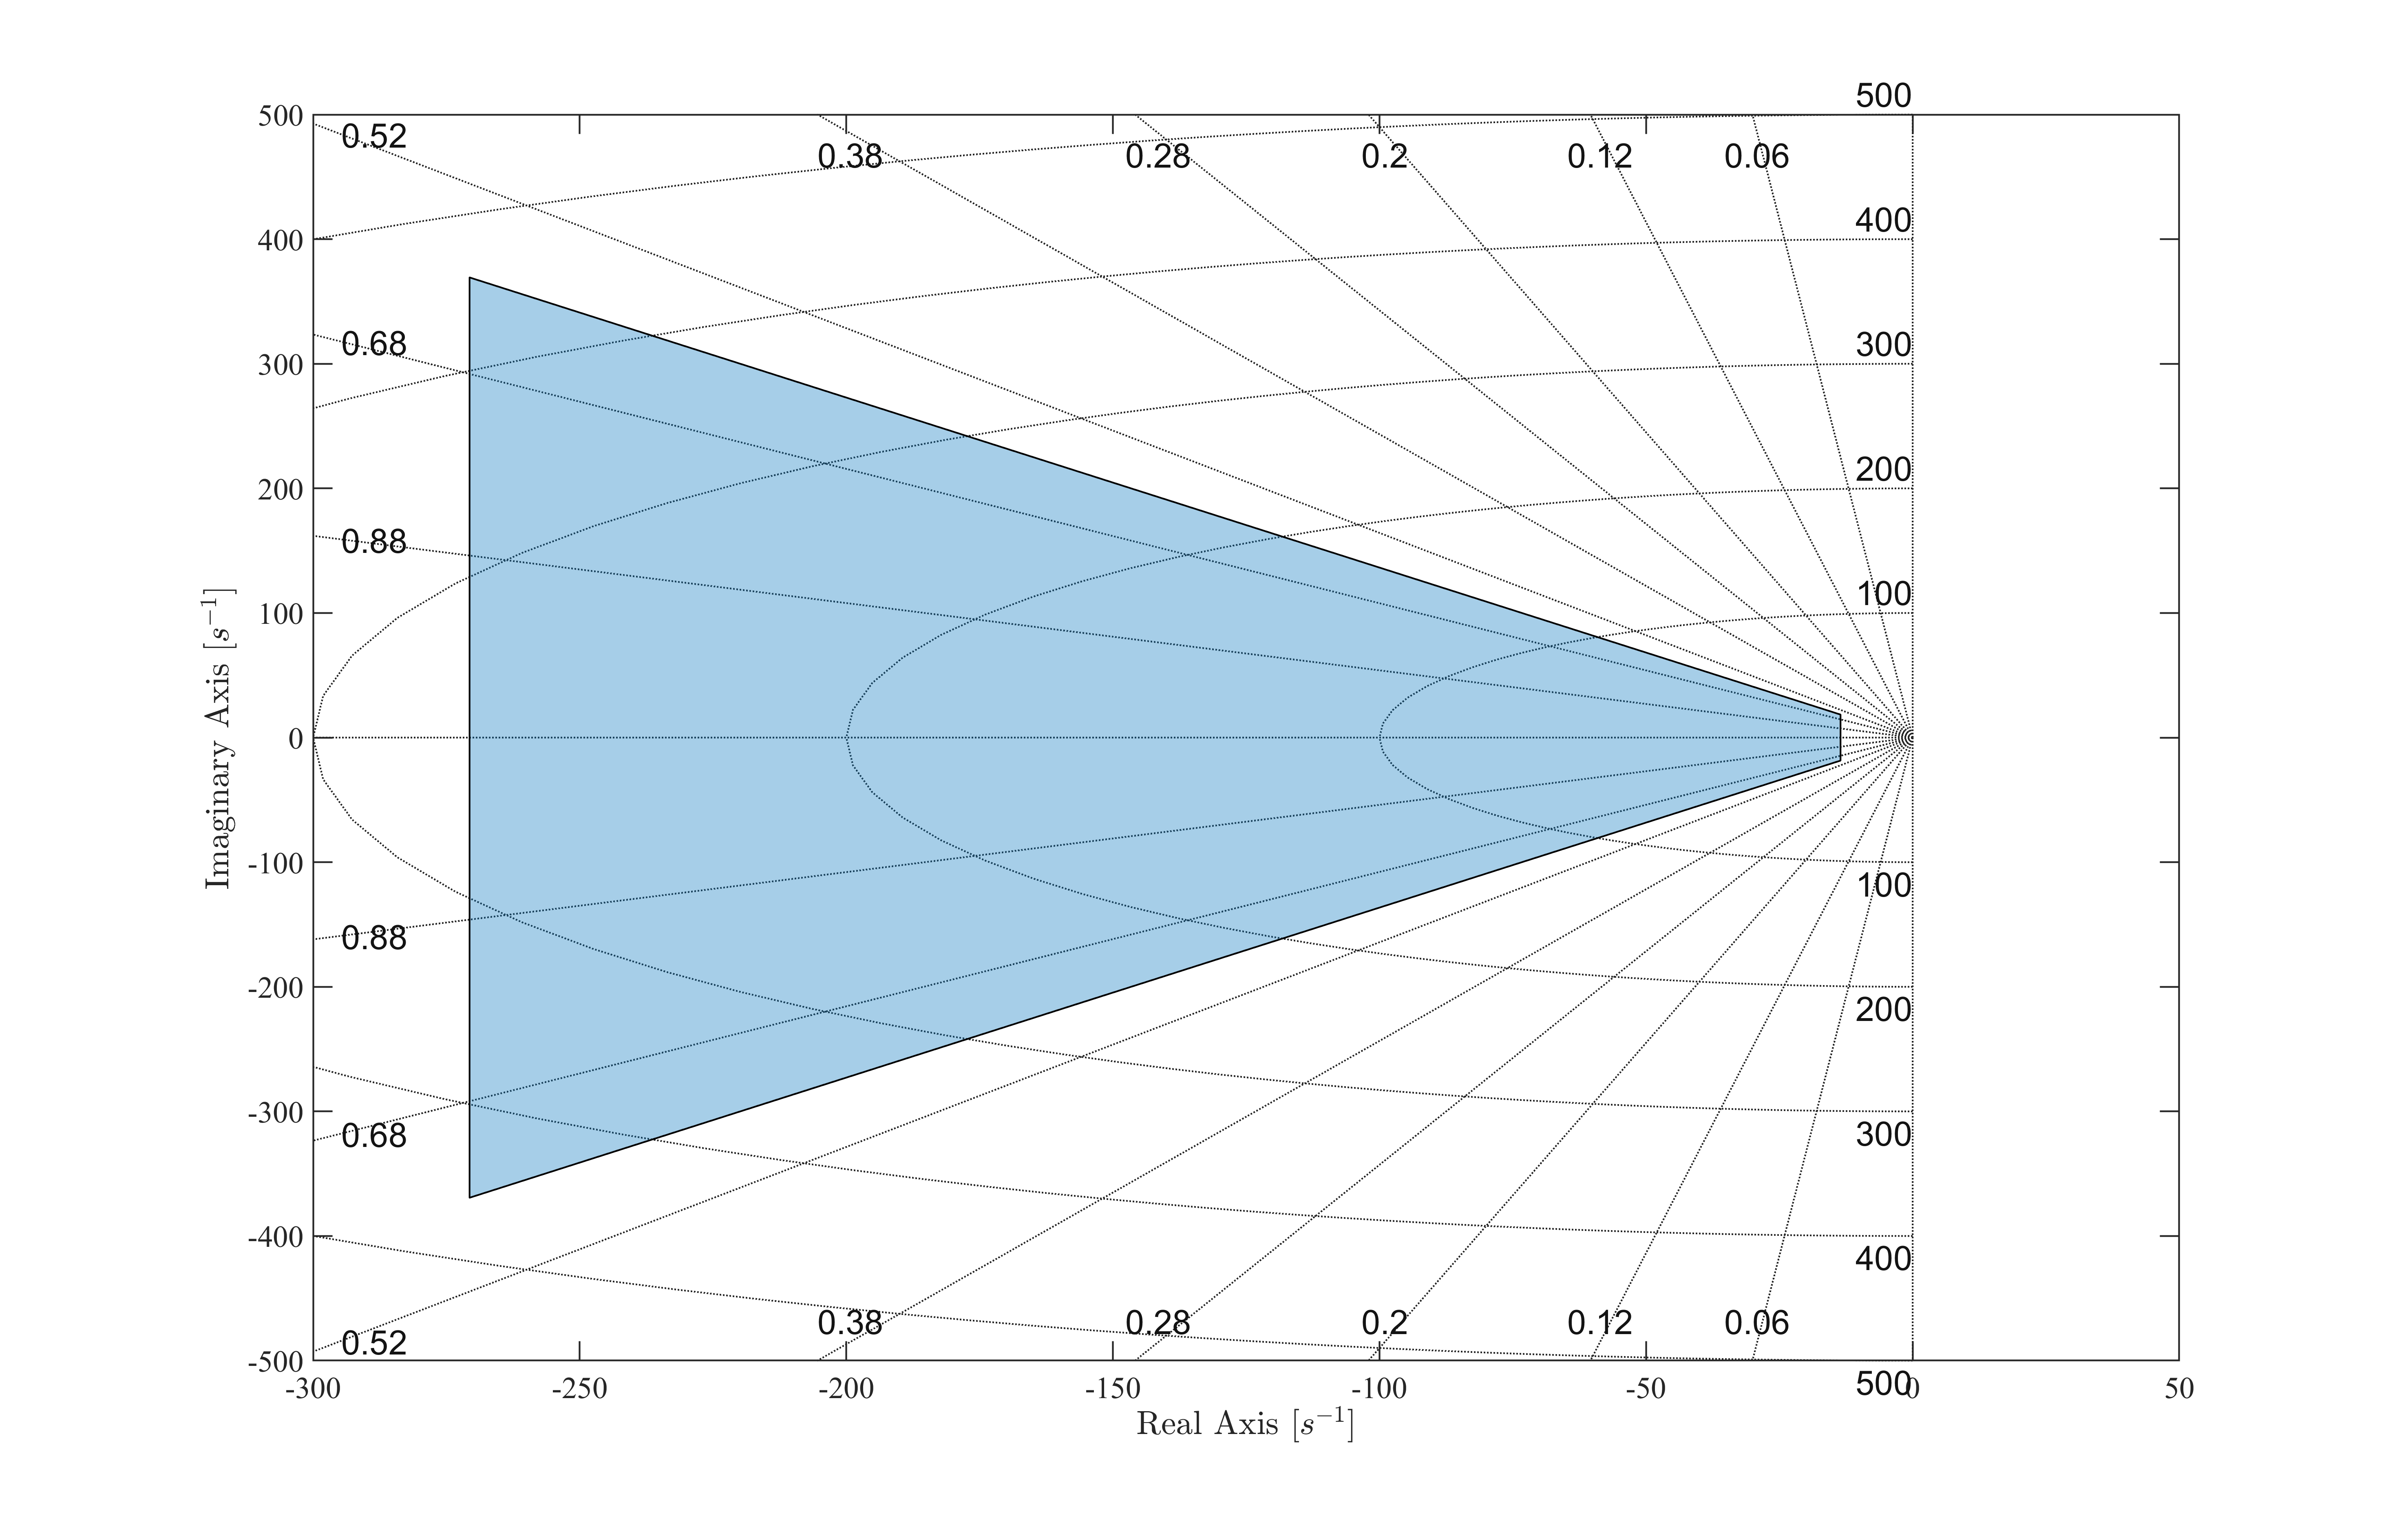
\includegraphics[width=7.5cm]{img/regiao_d_estabilidade.png}
    \caption{Região definida de estabilidade}
    \label{eq:dsta:regiaodef}
  \end{centering}
\end{figure}
\FloatBarrier

\subsection{Controlador Robusto por realimentação de estados com \( \mathcal{D}\)-estabilidade garantida}
Considerando o sistema no espaço de estados apresentado em \eqref{eq:dsta:linsys} com incerteza paramétrica nas matrizes $A$ e $B$, cujos valores são apresentados em \eqref{ed:linsys:ALPV} e \eqref{ed:linsys:BLPV}, em que o parâmetro $\delta$ representa a incerteza do modelo associada a massa do veiculo de $\pm100kg$. A síntese do  controlador  robusto ́e  realizada  pela  resolução das LMIs \eqref{eq:dsta:lmis} e \eqref{eq:dsta:lmisaux} para os parâmetros da região de \( \mathcal{D}\)-estabilidade definidos em \eqref{ed:dstab:params}. Os ganhos obtidos do procedimento de otimização são exibidos abaixo com precisão de 4 casas decimais:

\begin{equation*} \label{eq:ganhoscontrolador}
    K^'=
    \begin{bmatrix}
        -514929.0792&\\	
        -51637.9194&\\	
        791876.7347&\\
        2492.4857&\\
    \end{bmatrix}
\end{equation*}

Calculou-se a localização dos autovalores do sistema para os valores de $\delta = -100, -90, \dots, 90, 100$ e os resultados são exibidos na figura abaixo, com o sistema em malha aberta e malha fechada.
\FloatBarrier
\begin{figure}[htbp]
    \begin{centering}
    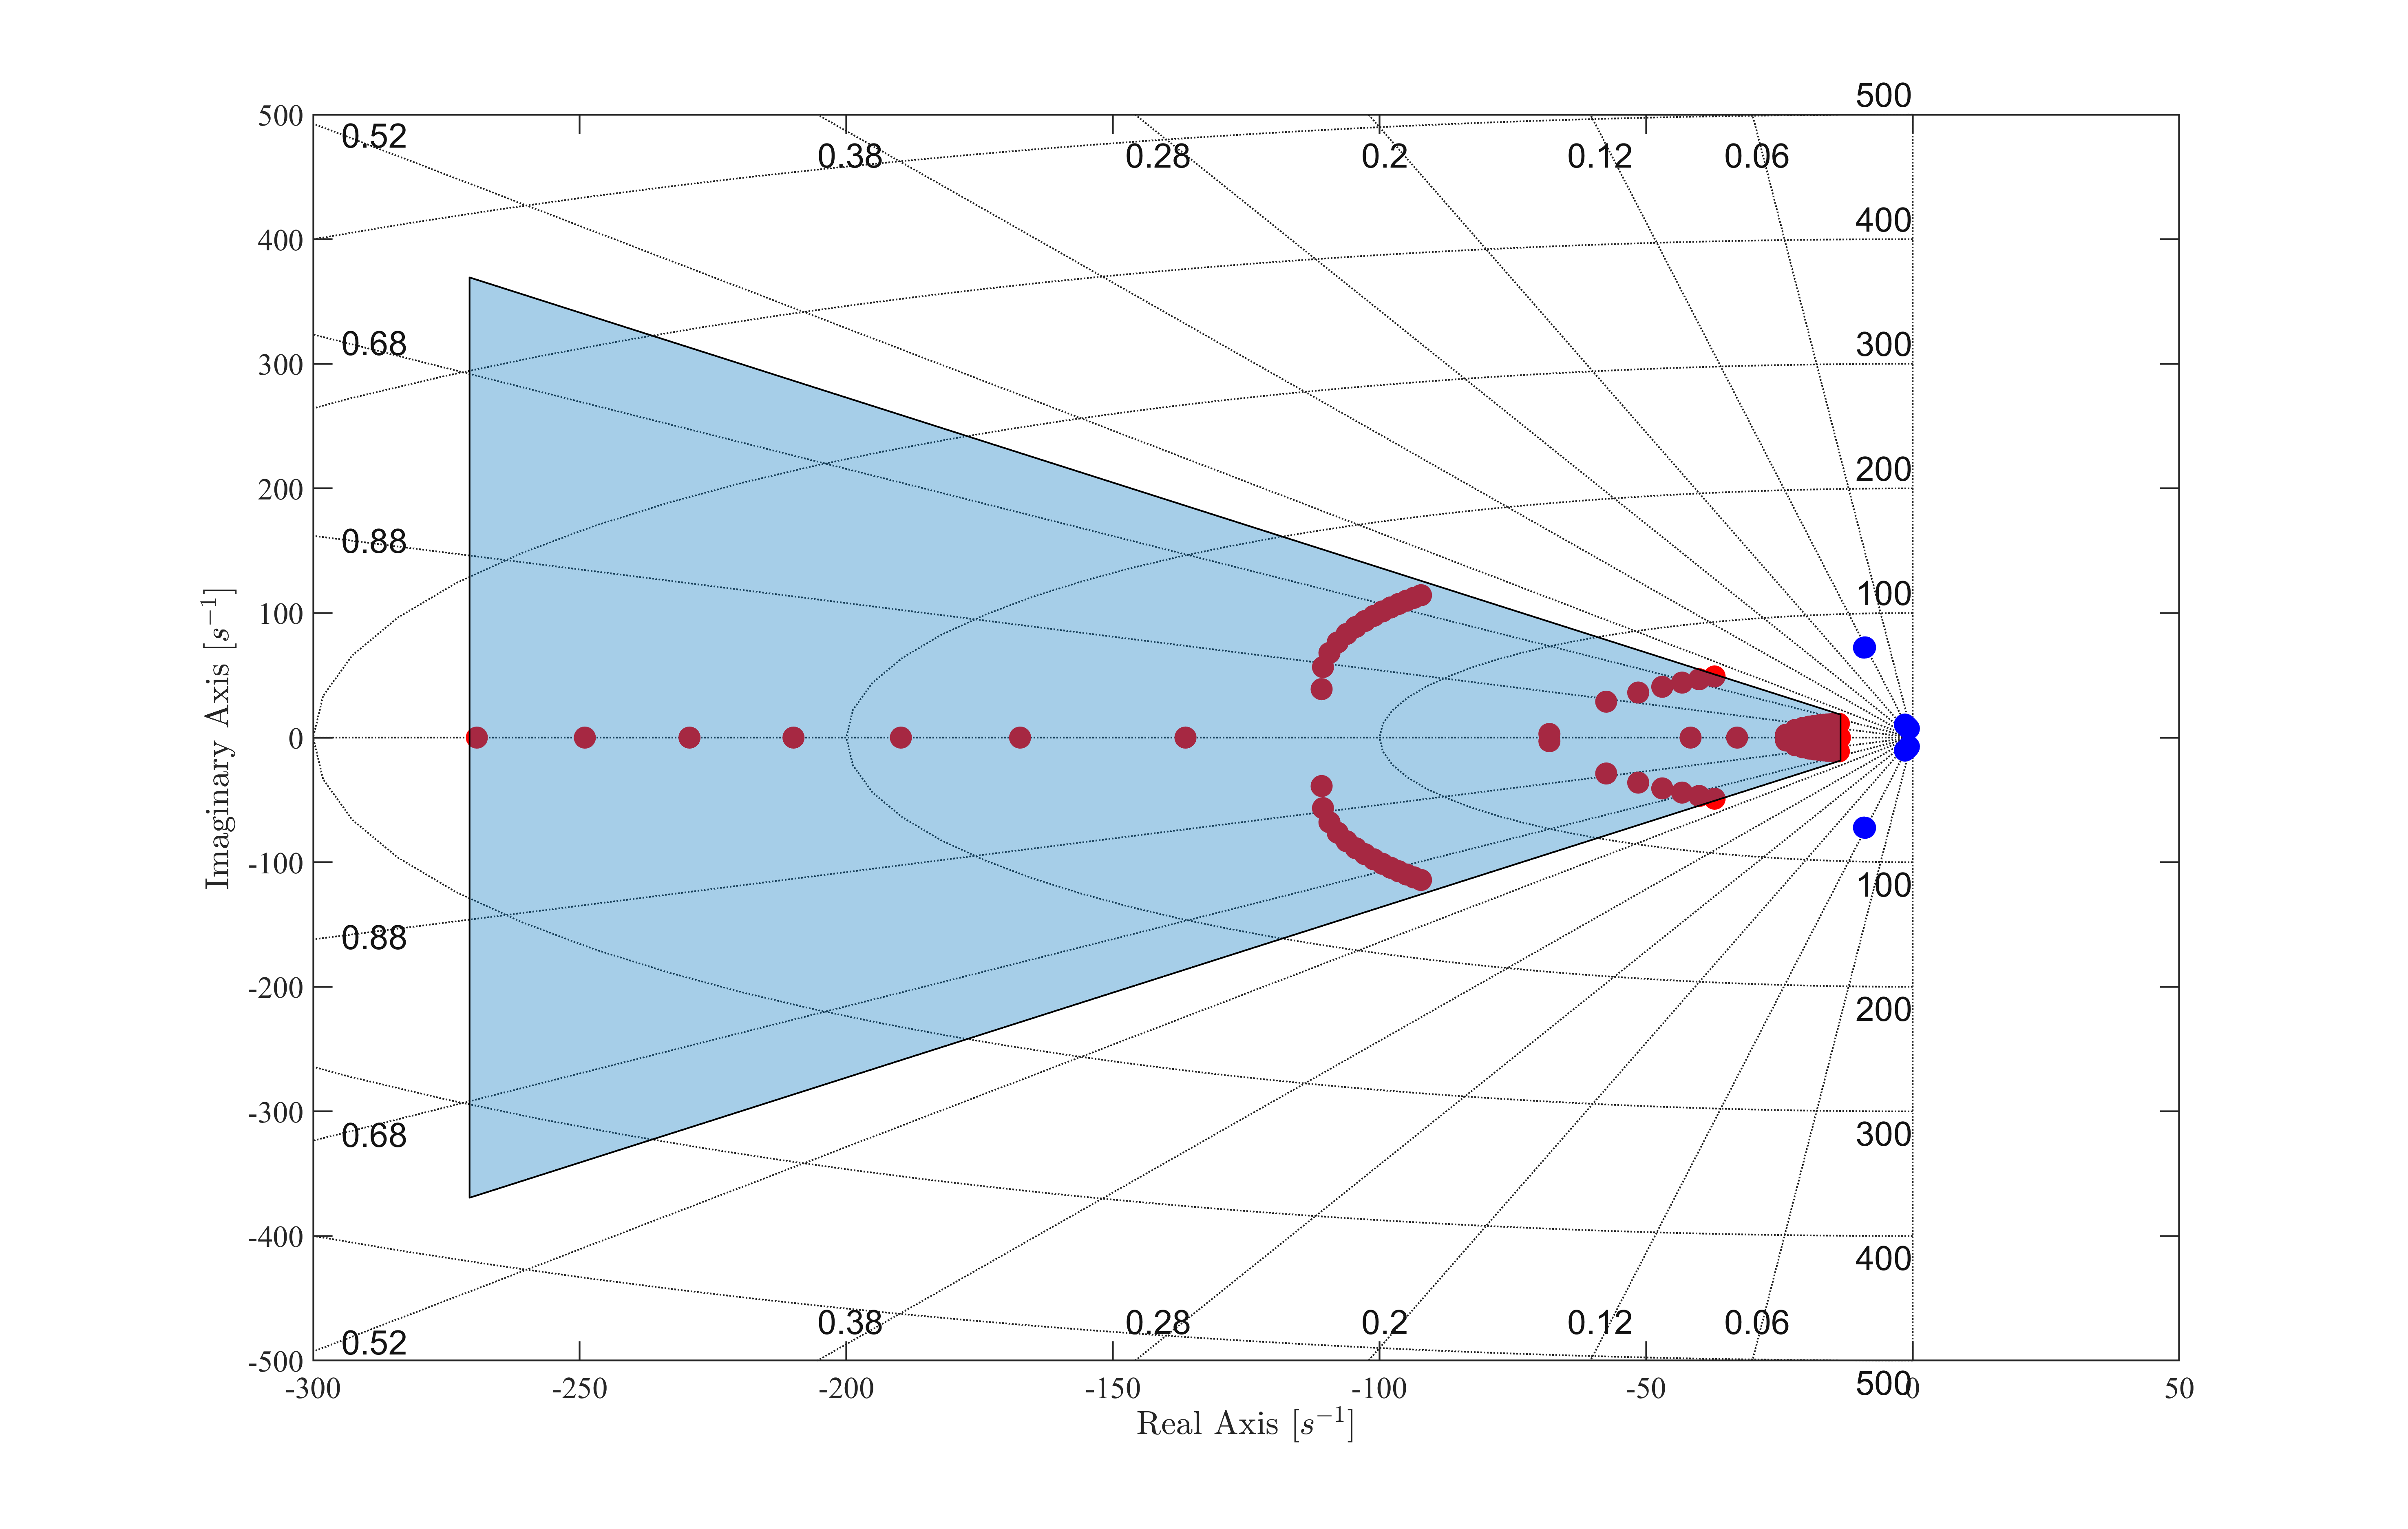
\includegraphics[width=7.5cm]{img/regiao_d_estabilidade_autoval.png}
    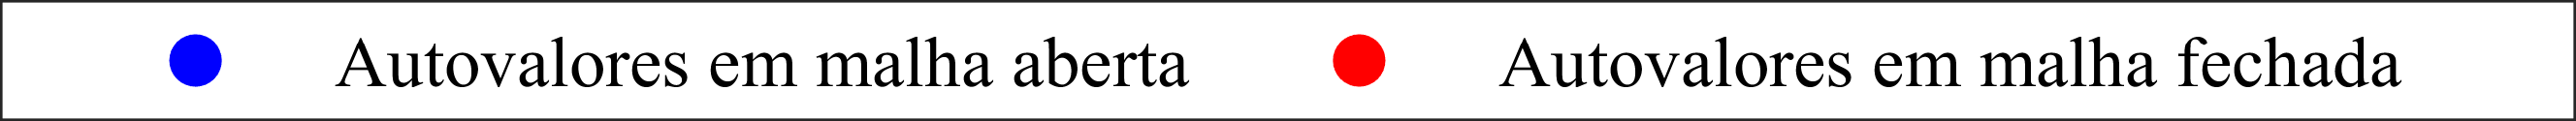
\includegraphics[width=6cm]{img/regiao_d_estabilidade_autoval_leg.png}
    \caption{Autovalores do sistema}
    \label{fig:regiao_d_estabilidade_autoval_leg}
    \end{centering}
\end{figure}
\FloatBarrier

Ao analisar o gráfico, nota-se que o controlador projetado foi capaz de manter os autovalores responsáveis pela resposta dinâmica do sistema em malha fechada dentro da região de \( \mathcal{D}\)-estabilidade para todos os valores testados do parâmetro $\delta$, sendo então um controlador com requsitos de desempenho temporal garantido.
\subsection{Observador de Luenberger}
Foi decidido que a dinâmica do estimador de estados deve ser 3 vezes  mais rápida do que a dinâmica do sistema em malha fechada, Foi adicionado o valor de $\beta_p=-270.6566$ como offset aos autovalores da planta original.
Estes foram utilizados para definir o conjunto de ganhos $L$ do observador de estados através da fórmula de Lyapunov definida em \eqref{eq:lyapunov}. 
Desta maneira, foi encontrada a seguinte matriz de ganhos de realimentação para o observador de estados linear, números arredondados na quarta casa decimal:

\begin{equation} \label{eq:ganhos_pred} \small
    \begin{split}
        \mathbf{L}=\
    \end{split}
    \begin{bmatrix}
       -14634.2594& -14634.2594& -14634.2594& -14634.2594&\\
        23918.8824&  23918.8824&  23918.8824&  23918.8824&\\
        -1401.1937&  -1401.1937&  -1401.1937&  -1401.1937&\\
        -6800.803 &  -6800.803 &  -6800.803 &  -6800.803 &\\
    \end{bmatrix}
\end{equation}

Uma simulação temporal do sistema linear controlado pelo ganho de realimentação de estados, obtido através do preditor desenvolvido nesta seção é exibido nas figuras a seguir. Para isso considerou-se o sistema operando na condição nominal com $\delta=0$, em malha aberta, e uma entrada de perturbação dada por:

\begin{equation}\label{eq:estatdos_perturbacao} \footnotesize
    \omega(t)=0.6sin(8\pi t)+0.75sin(12\pi t)+0.9sin(16\pi t)+0.5sin(20\pi t)
\end{equation}

\FloatBarrier
\begin{figure}[htbp]
    \begin{centering}
    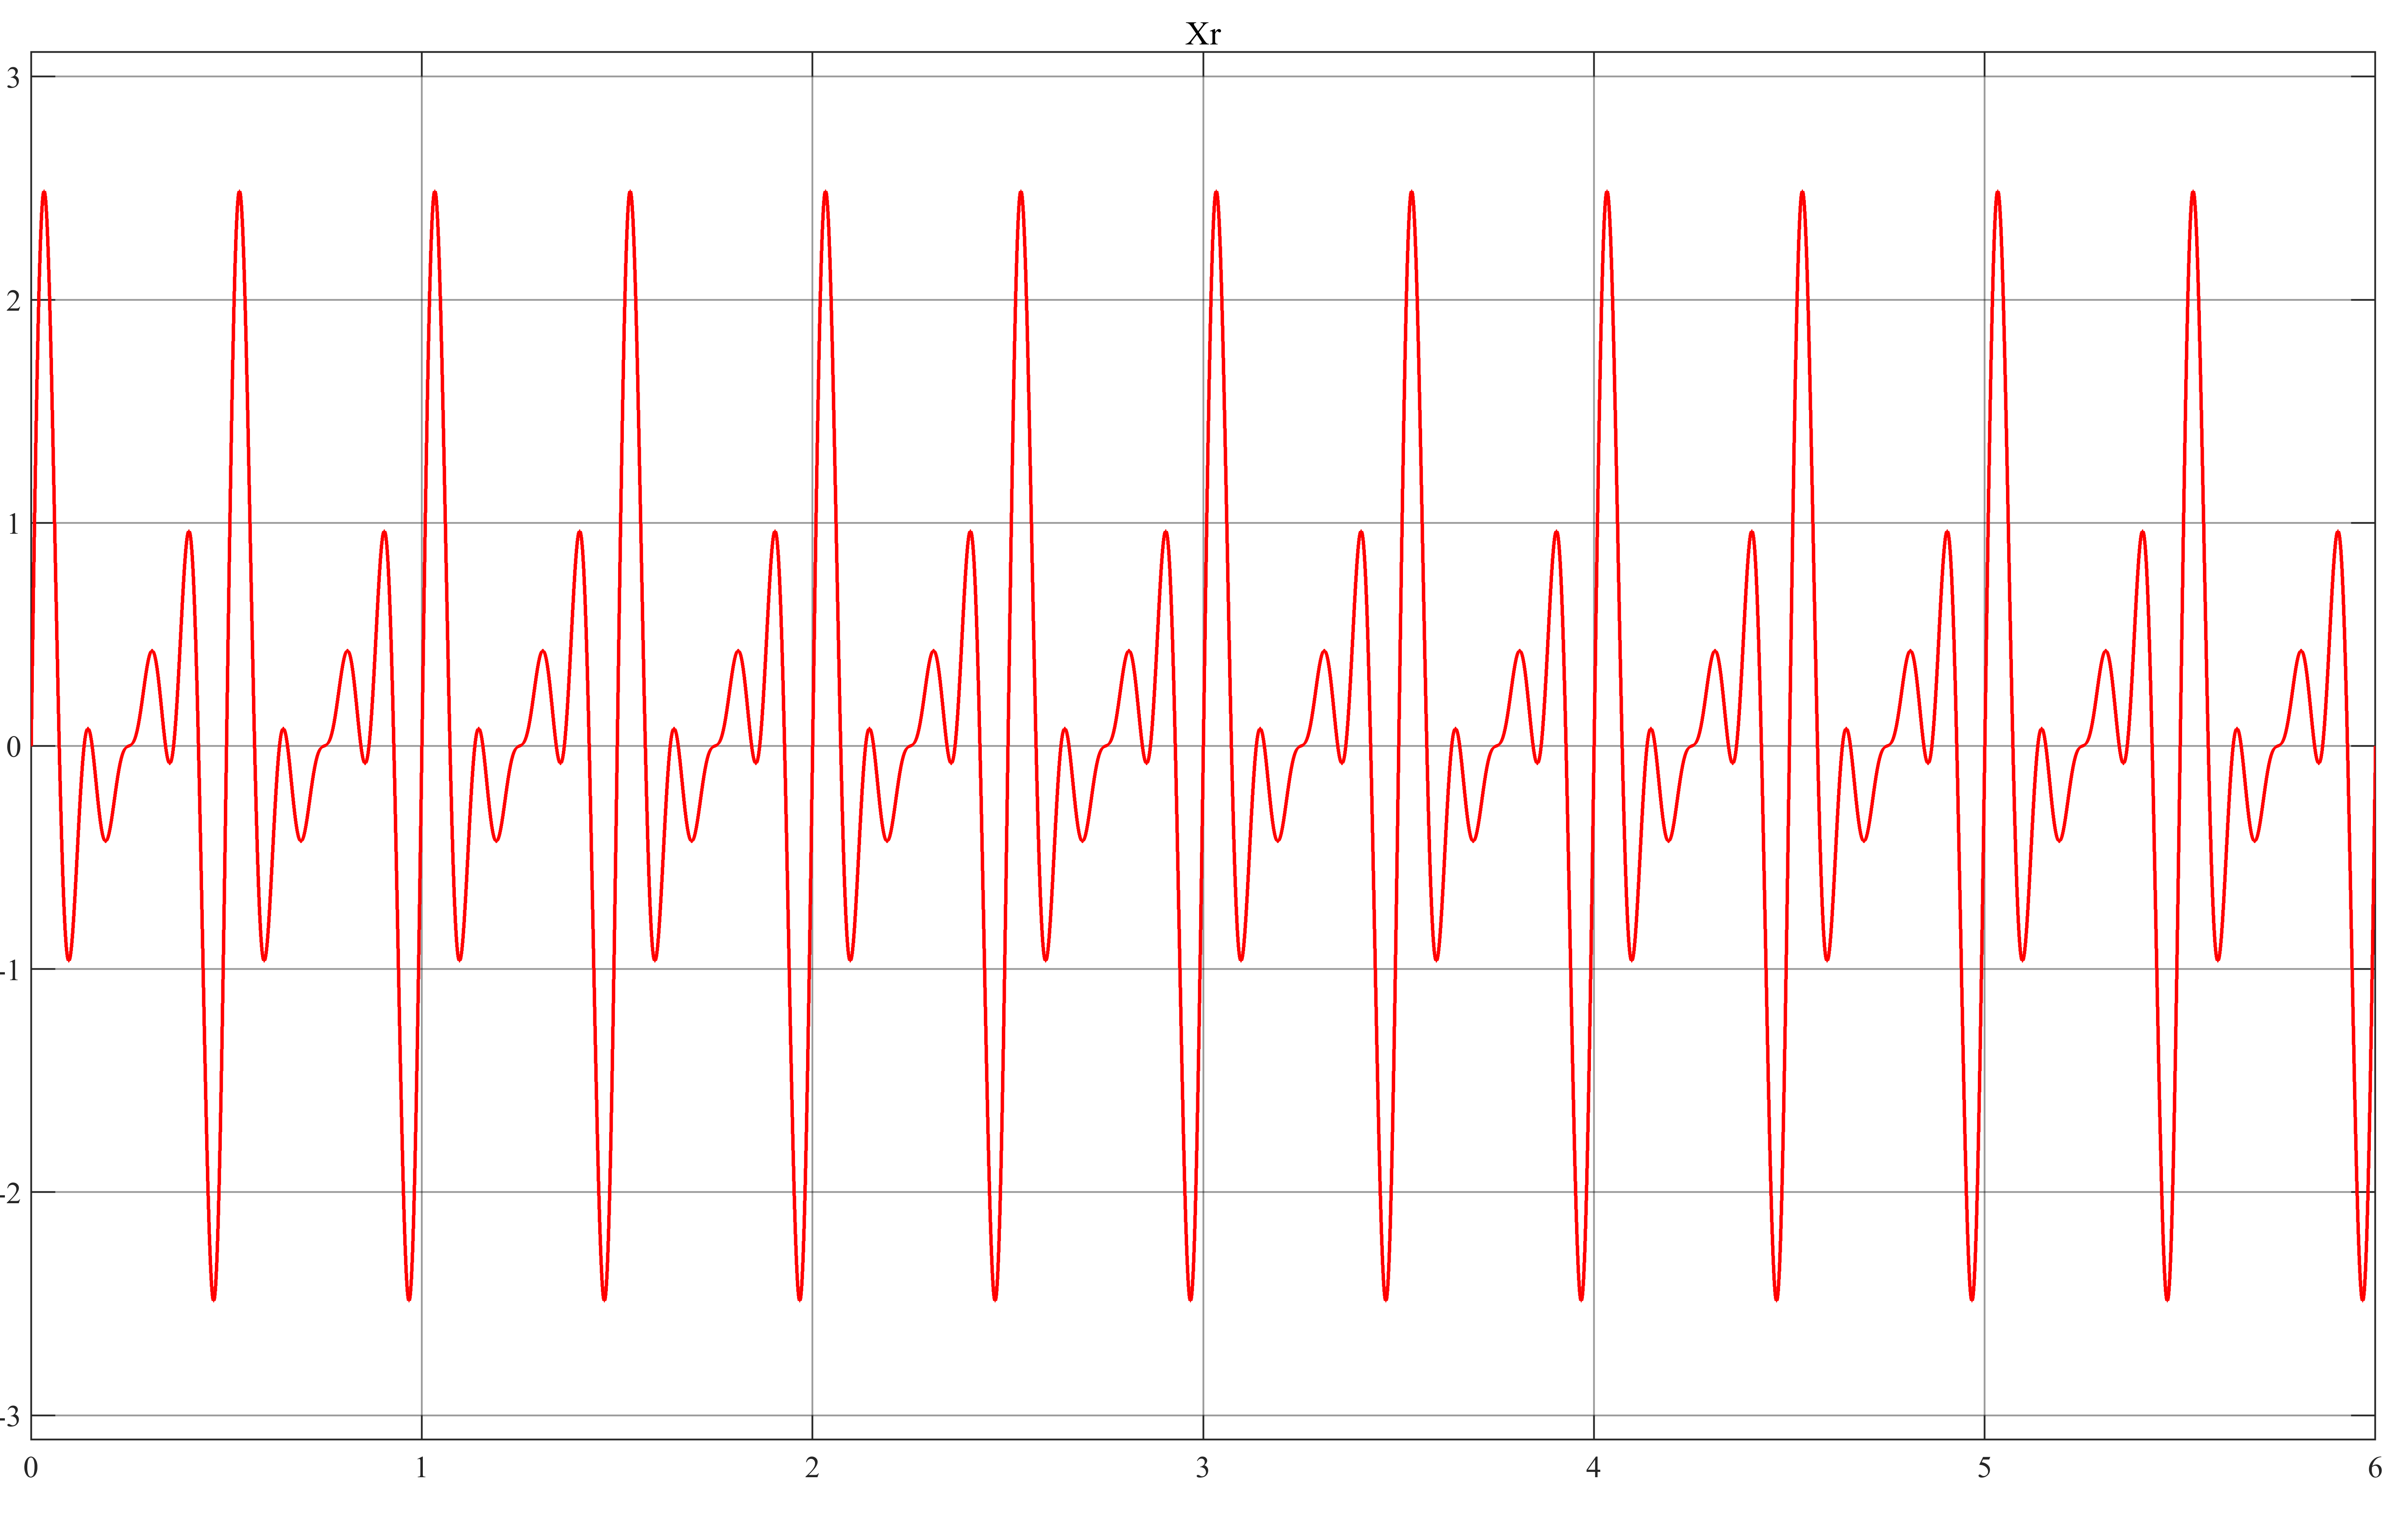
\includegraphics[width=7.5cm]{img/estatdos_perturbacao.png} 
    \caption{Perturbação para teste do observador}
    \label{fig:estatdos_perturbacao}
    \end{centering}
\end{figure}
\FloatBarrier

A figuras \ref{fig:estatdos_luenberger} a seguir mostram a evolução dos estados reais e preditos enquanto a figura \ref{fig:estatdos_erro_luenberg} mostra o erro de predição dos estados.

\FloatBarrier
\begin{figure}[htbp]
    \begin{centering}
    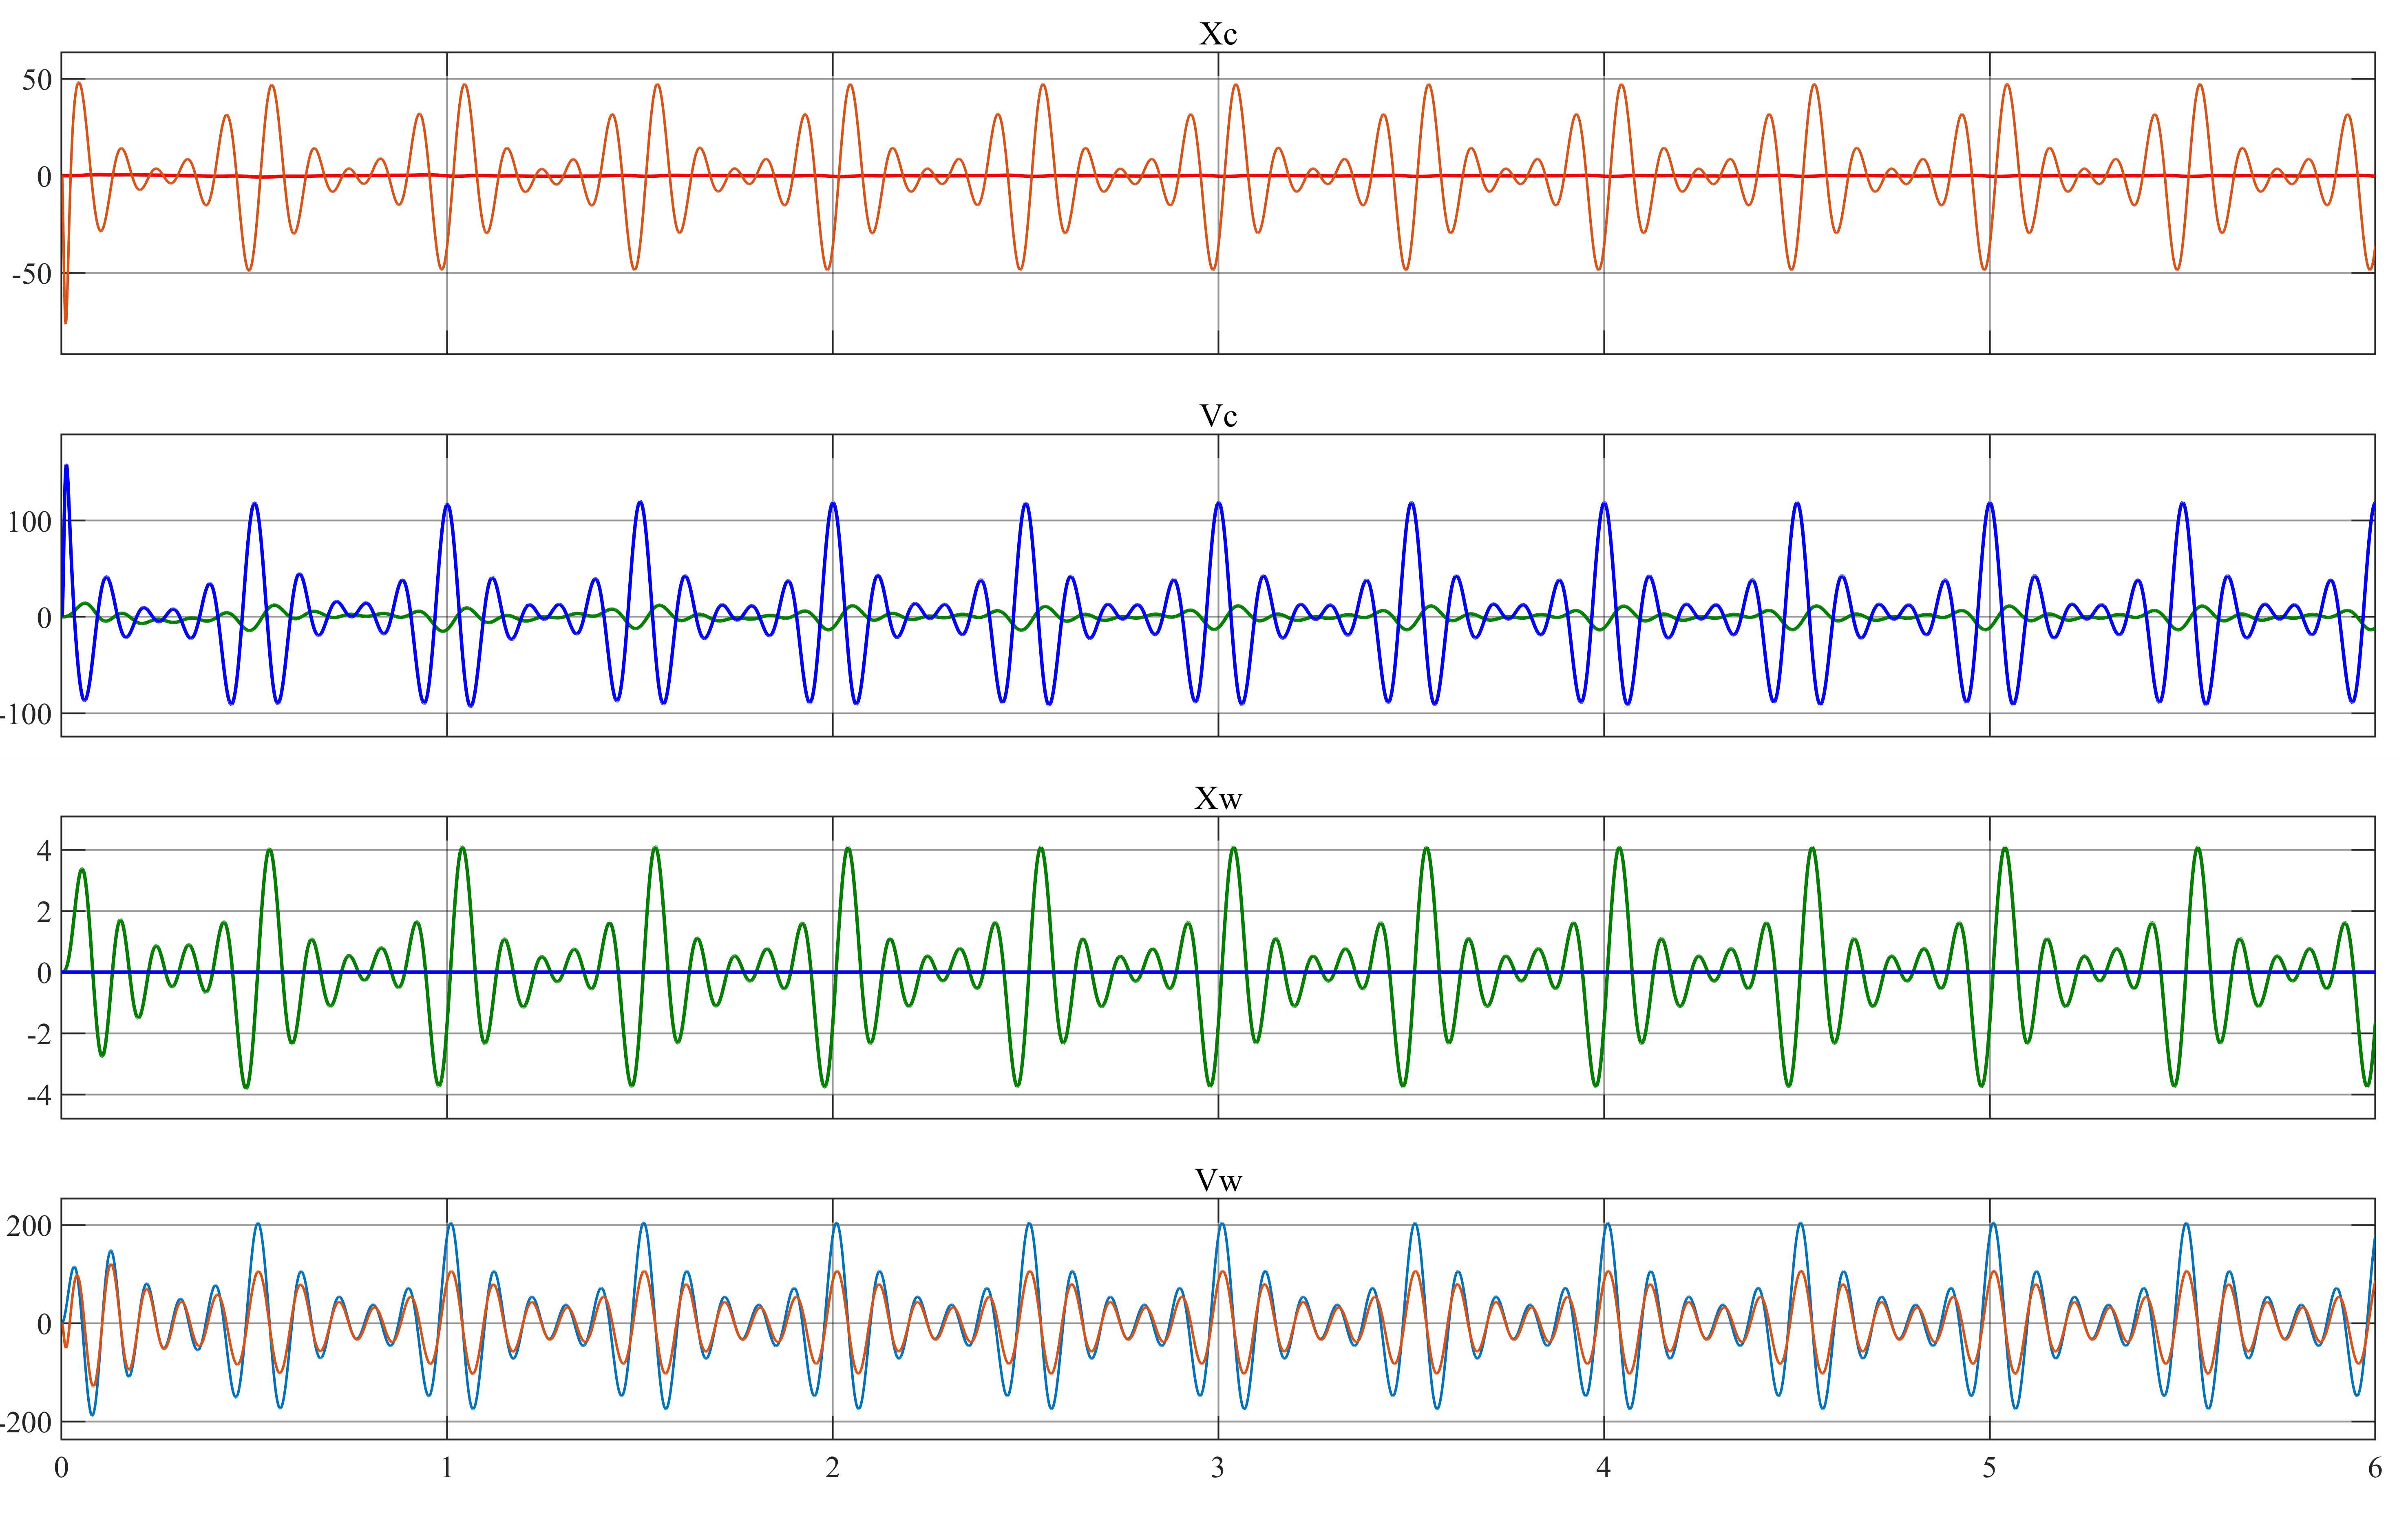
\includegraphics[width=7.5cm]{img/estatdos_luenberger.png} 
    \caption{Comparação dos estados do sistema com o observador de Luenberger}
    \label{fig:estatdos_luenberger}
    \end{centering}
\end{figure}
\FloatBarrier

\FloatBarrier
\begin{figure}[htbp]
    \begin{centering}
    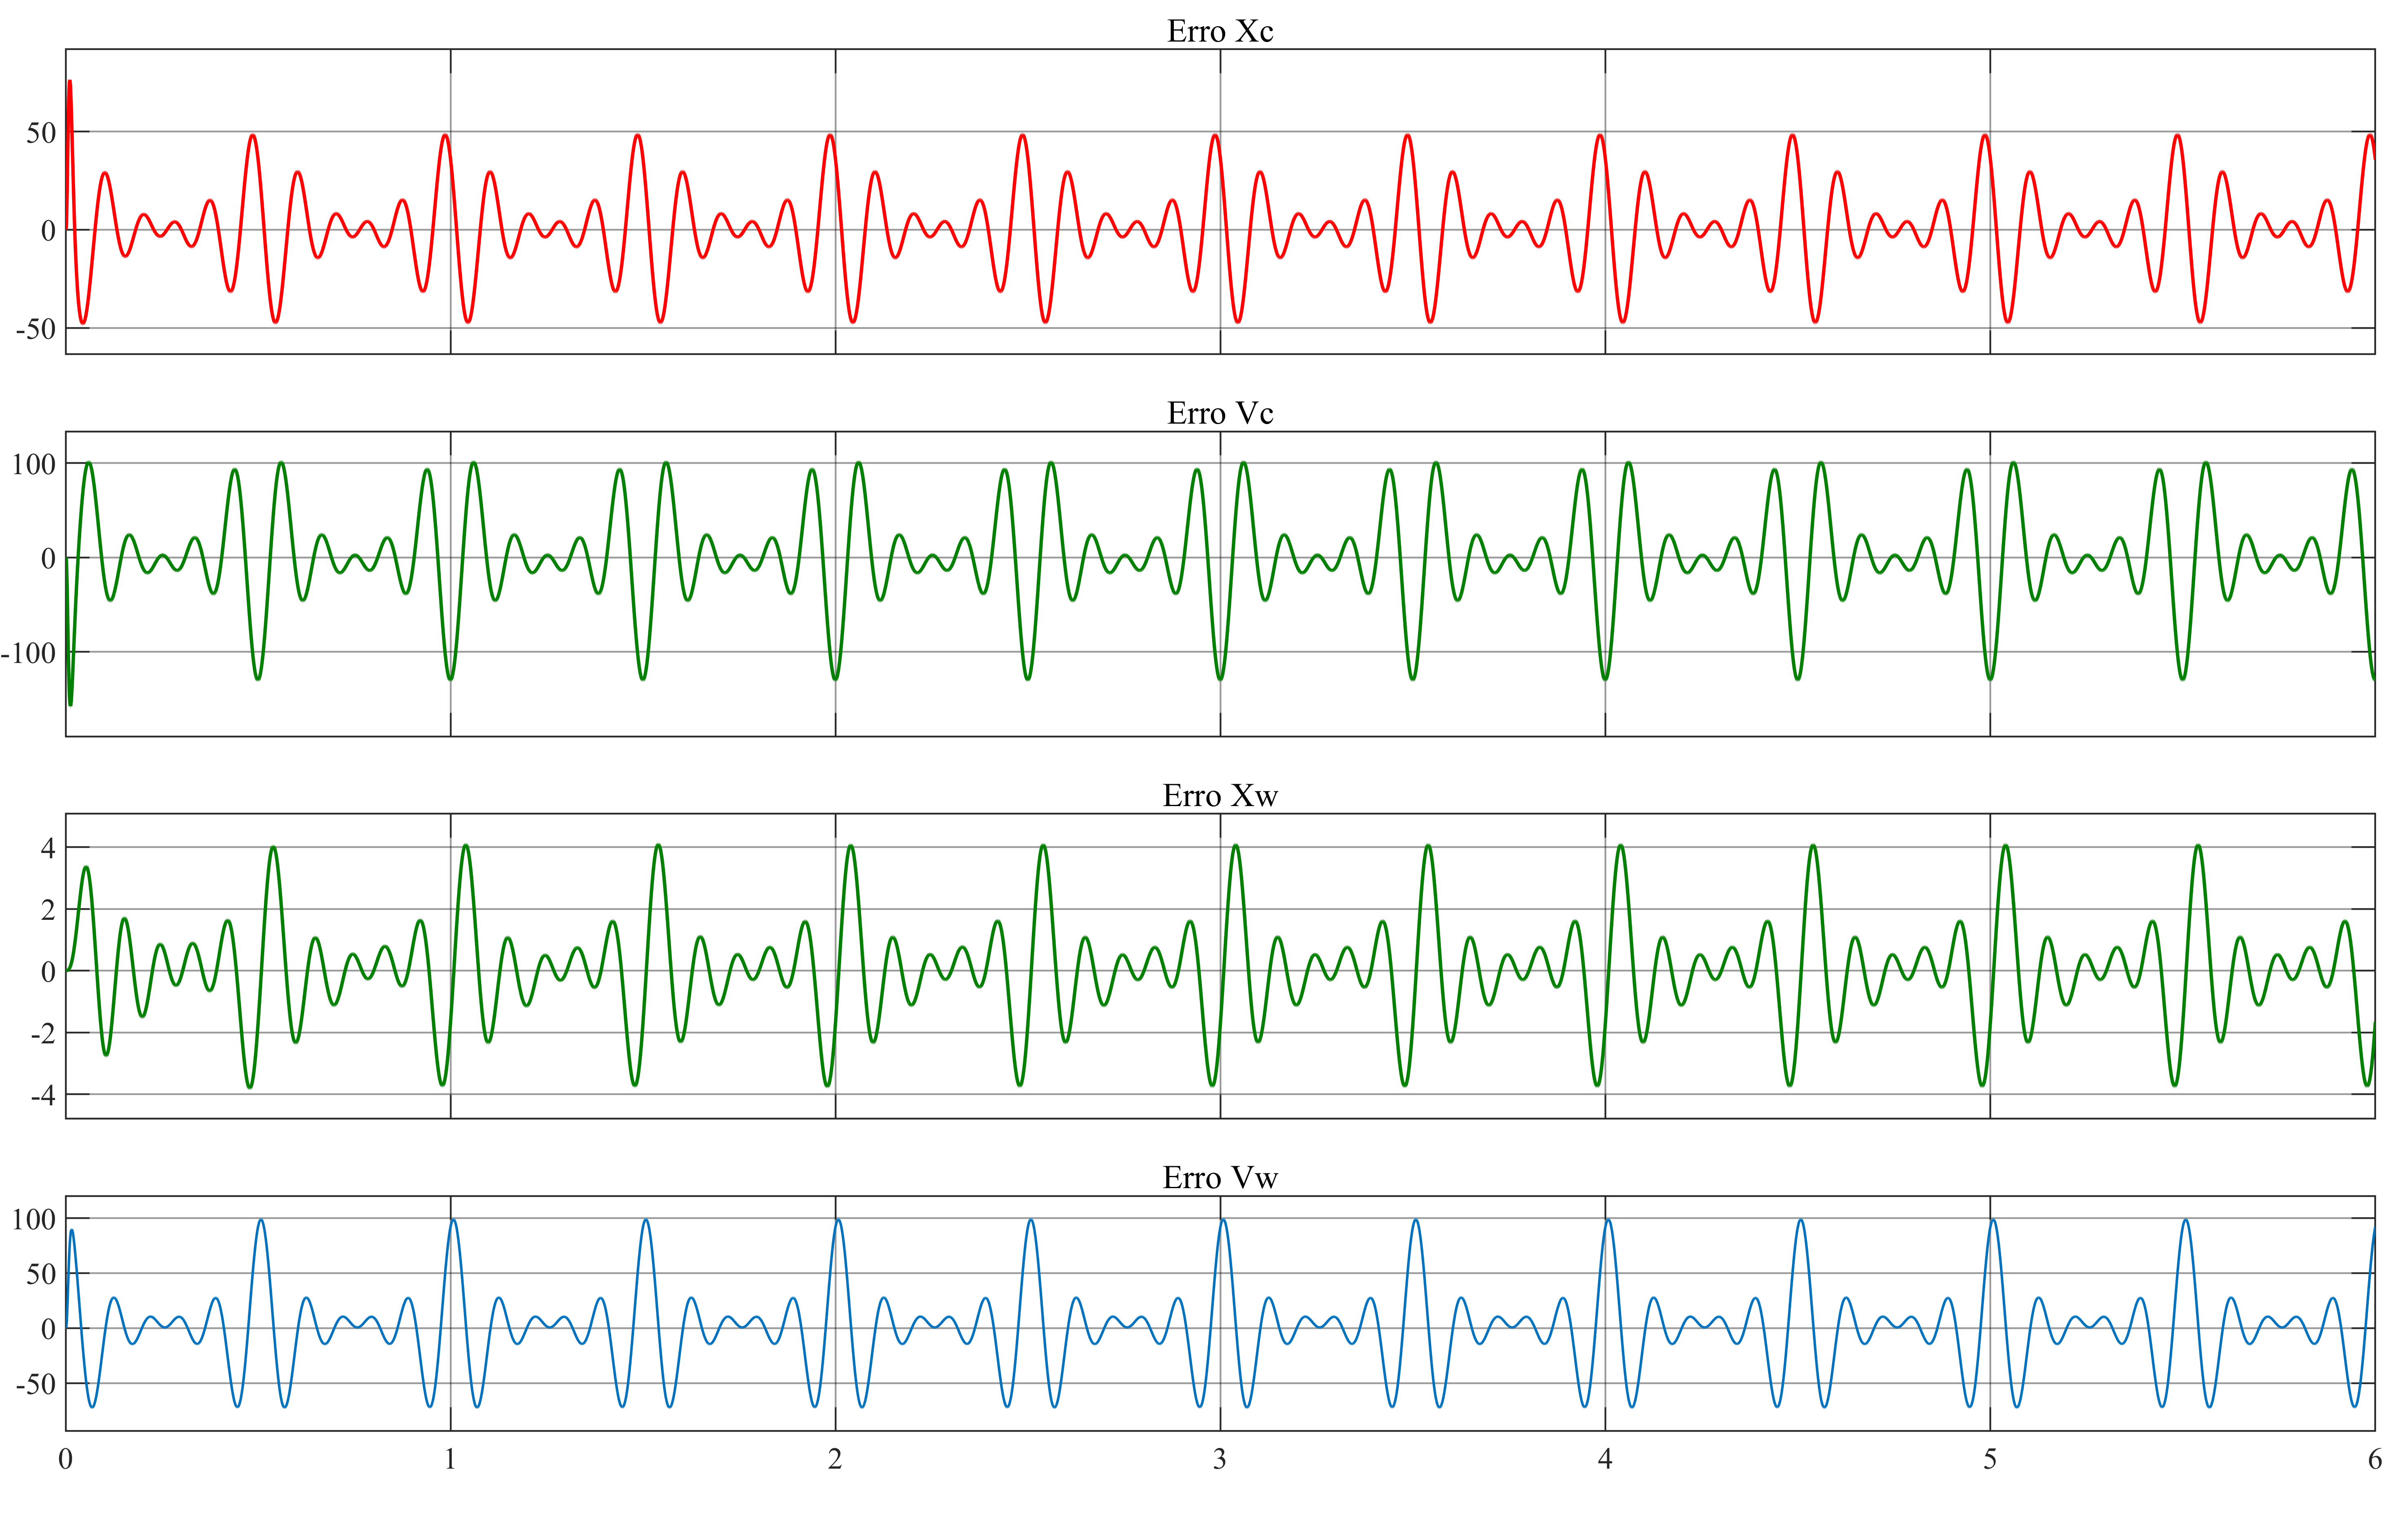
\includegraphics[width=7.5cm]{img/estatdos_erro_luenberg.png} 
    \caption{Erro do observador de Luenberger}
    \label{fig:estatdos_erro_luenberg}
    \end{centering}
\end{figure}
\FloatBarrier

\subsection{Observador de entradas desconhecidas}
Aplicando o Teorema \ref{theo:UIO}, obteve-se um limitante $\gamma=2.9084\cdot10^{-5}$. Simulou-se o sistema em conjunto com o observador aplicando a mesma perturbação definida em \eqref{eq:estatdos_perturbacao}.
A figuras \ref{fig:estatdos_luenberger} a seguir mostram a evolução dos estados reais e preditos enquanto a figura \ref{fig:estatdos_erro_luenberg} mostra o erro de predição dos estados.

\FloatBarrier
\begin{figure}[htbp]
    \begin{centering}
    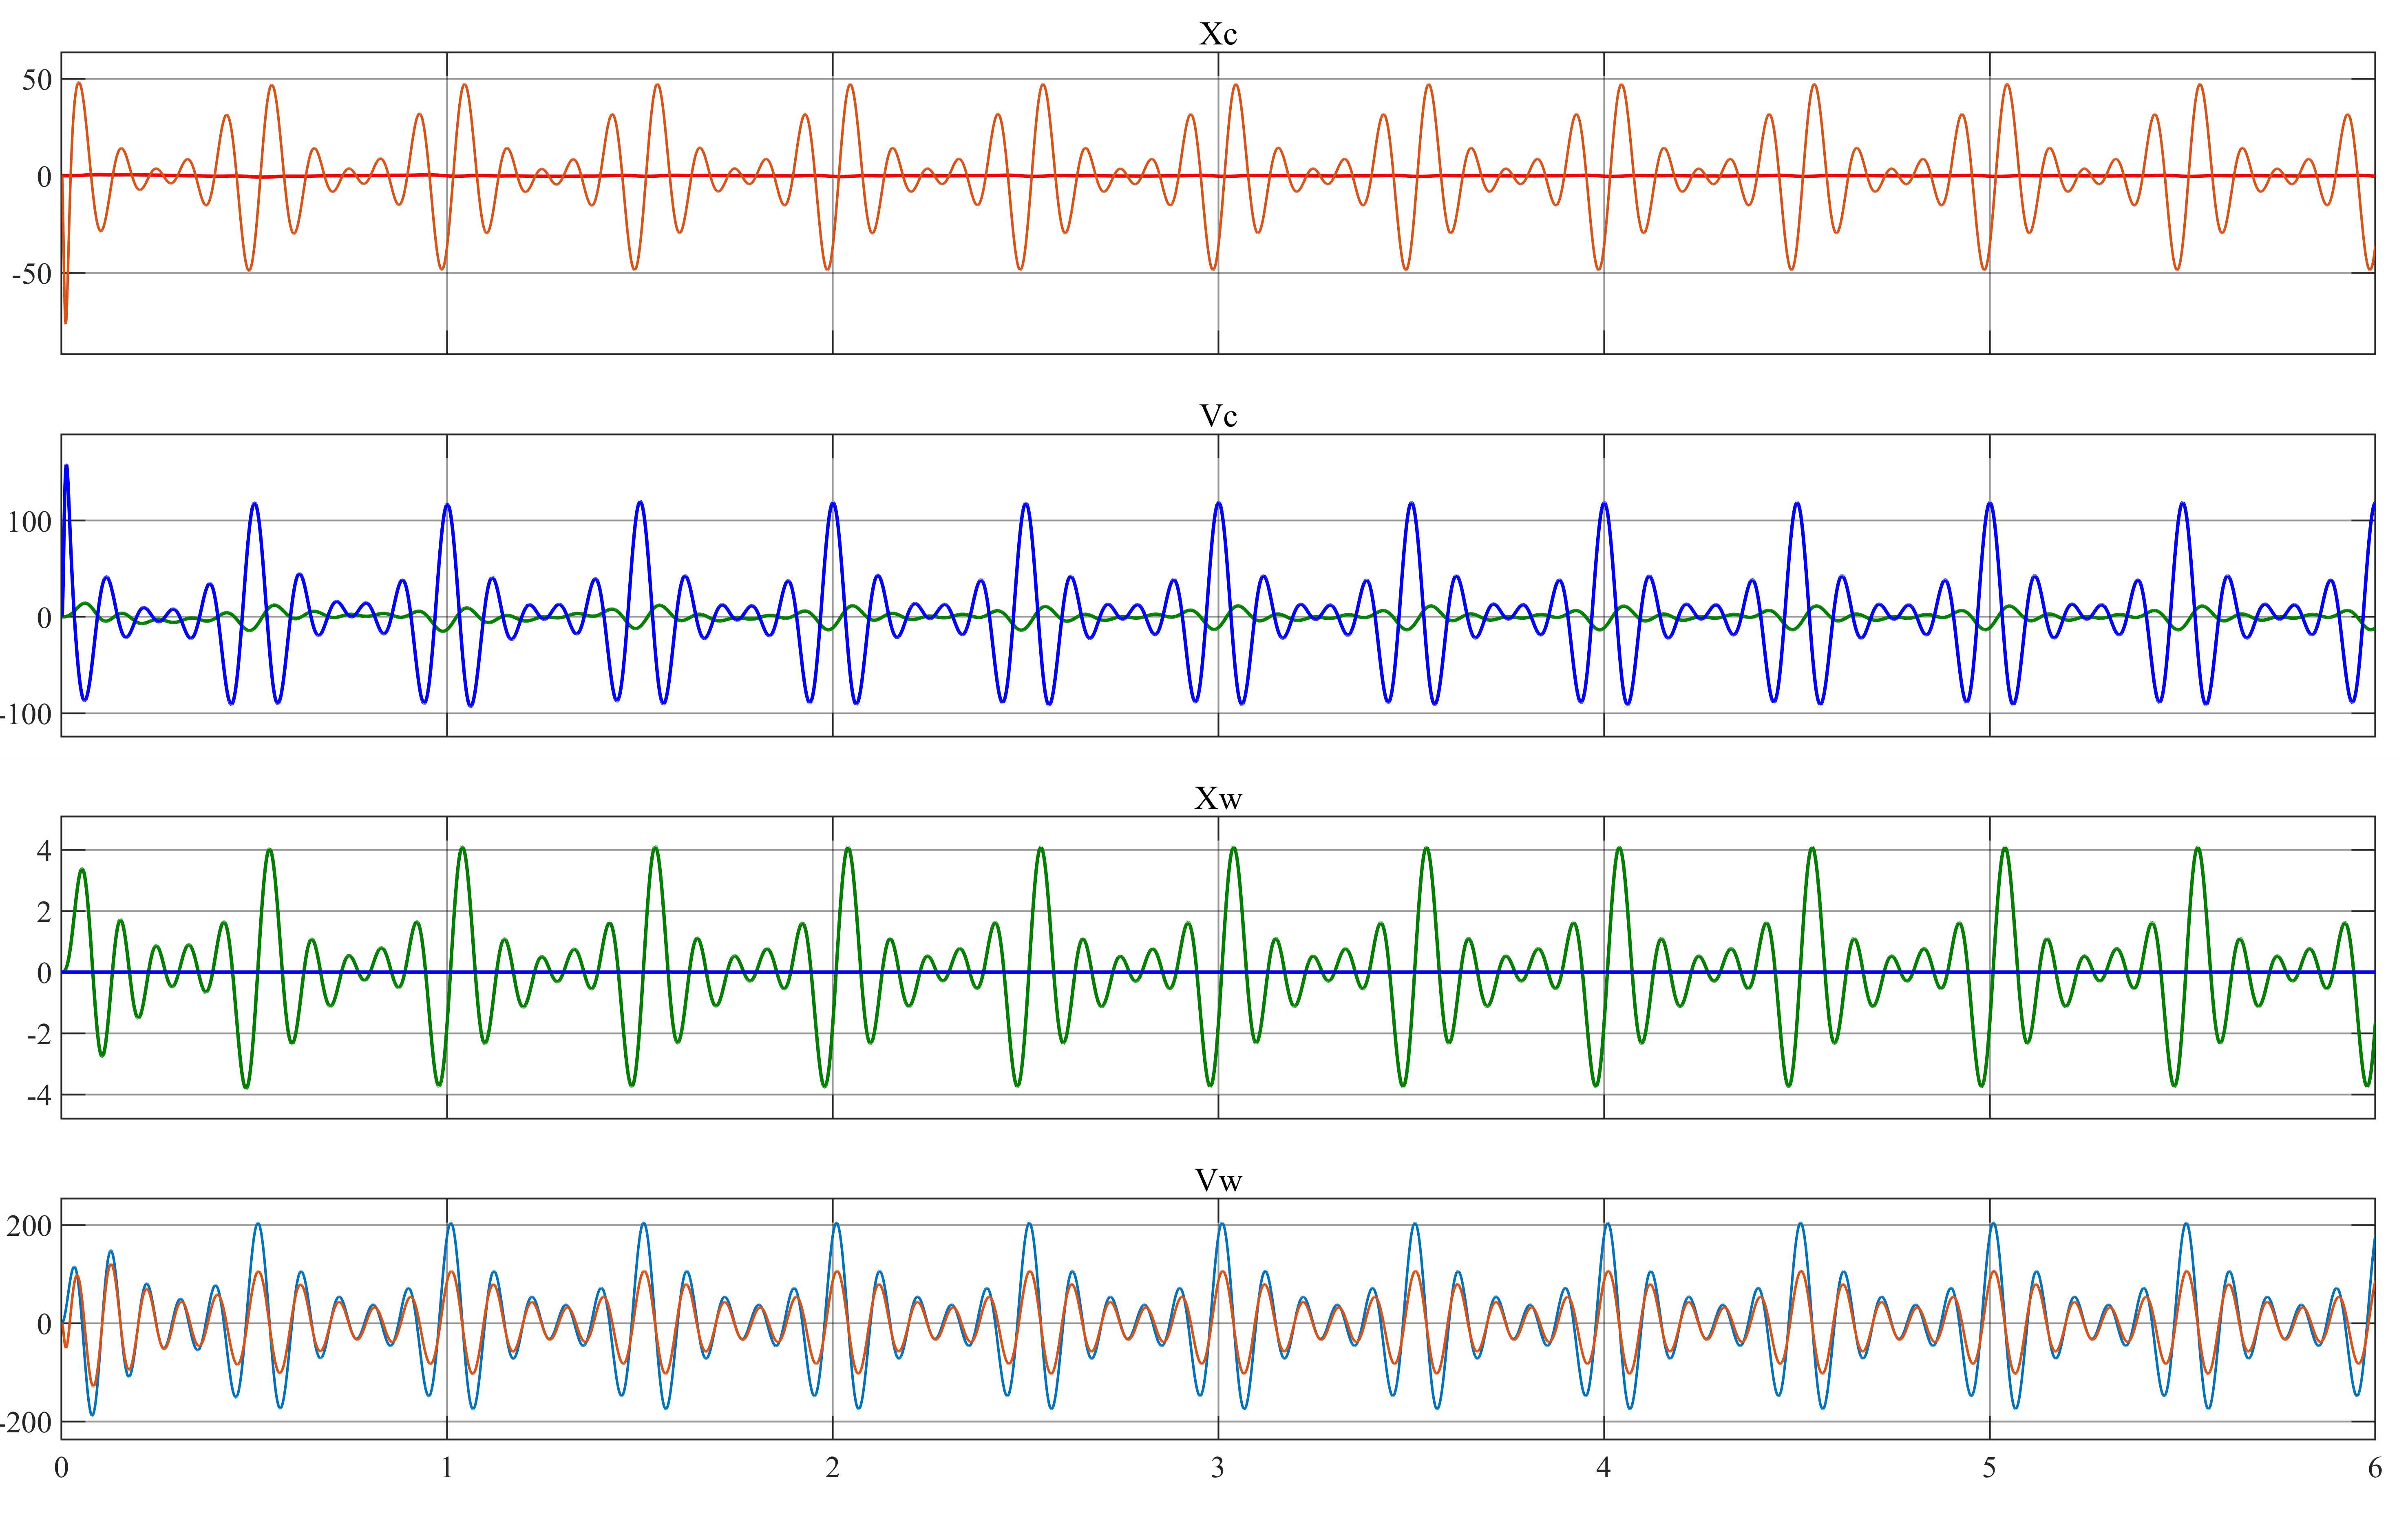
\includegraphics[width=7.5cm]{img/estatdos_luenberger.png} 
    \caption{Comparação dos estados do sistema com o observador de Luenberger}
    \label{fig:estatdos_luenberger}
    \end{centering}
\end{figure}
\FloatBarrier

\FloatBarrier
\begin{figure}[htbp]
    \begin{centering}
    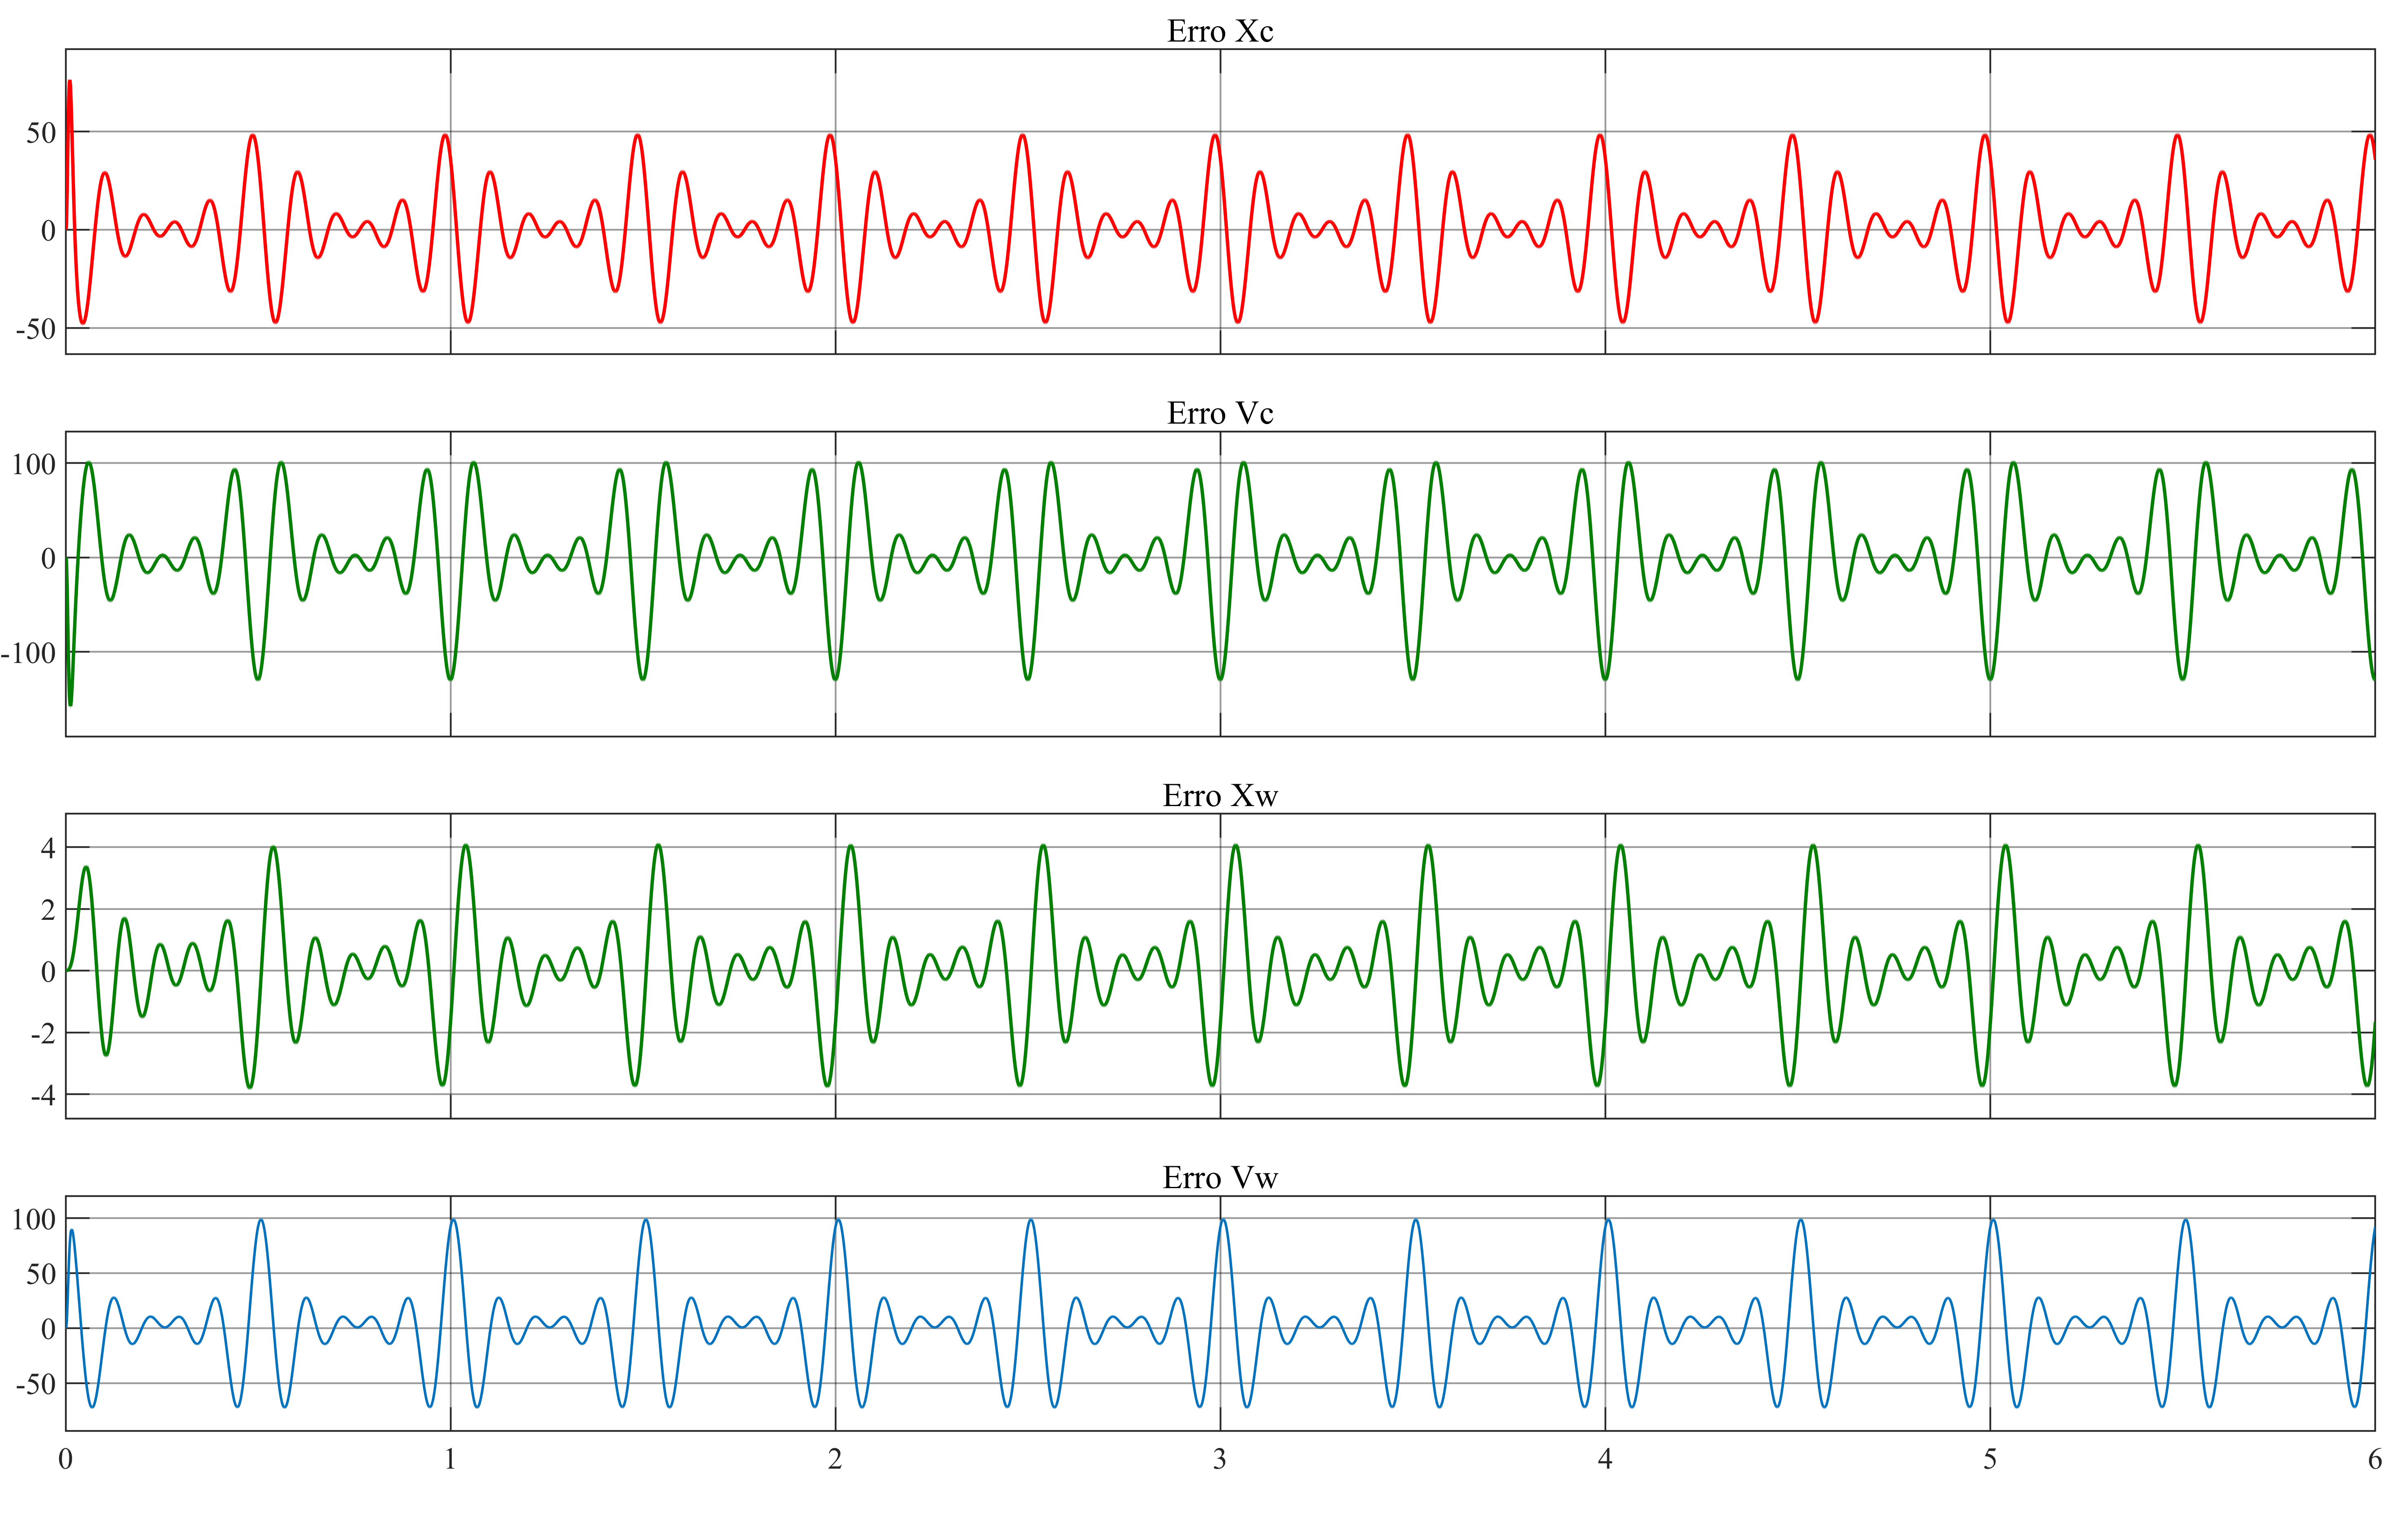
\includegraphics[width=7.5cm]{img/estatdos_erro_luenberg.png} 
    \caption{Erro do observador de Luenberger}
    \label{fig:estatdos_erro_luenberg}
    \end{centering}
\end{figure}
\FloatBarrier